\documentclass{article}
\usepackage[utf8]{inputenc}
\usepackage[spanish]{babel}
\usepackage{graphicx}	%Si se quiere compilar con las imagenes
% \usepackage[draft]{graphicx}	%Si NO se quiere compilar con las imagenes porque tarda mucho
\usepackage{graphics, float, fancyhdr, titling, caption, subcaption}
\usepackage{listings}
\usepackage[a4paper, total={6in, 9.5in}]{geometry}
\usepackage{fancyhdr}
\usepackage{hyperref}   %para que funcione addcontentsline debe ser la ultima que se cargue

%\setcounter{secnumdepth}{-2}       %Poner solo esto si no se quieren numero delante de las secciones y niveles inferiores.

\renewcommand{\footrulewidth}{0.4pt}
\title{

\includegraphics[width=1.75in]{imagenes/UGR-Logo.png} \\
\vspace*{1in}
\textbf{Cuestiones Tema 3} \\
Animación por Ordenador \\
\vspace*{0.5in}}
\author{Andrés Merlo Trujillo \\
andresmerlo@correo.ugr.es \\
77147239H \\ 
\vspace*{0.5in} \\
E.T.S. de Ingenierías Informática y de Telecomunicación \\
\textbf{Universidad de Granada}} \date{\today}

\hypersetup{
    colorlinks=true,
    linkcolor=black,
    citecolor=black
}

\renewcommand\maketitlehooka{\null\mbox{}\vfill}
\renewcommand\maketitlehookd{\vfill\null}

\begin{document}
\begin{titlingpage}
\maketitle
\end{titlingpage}

\tableofcontents

\newpage

\pagestyle{fancy}   %a partir de comienza el header (se salta el indice y portada)
\fancyhead[L]{Andrés Merlo Trujillo}
\fancyhead[R]{Animación por Ordenador}
%\section{Ejercicio 1}
%\begin{figure}[H]
%    \centering
%    \includegraphics[width=\textwidth]{imagenes/passwdfile.png}
%    \vspace{10pt}
%    \footnotesize{Fuente: https://...}
%\end{figure}

% \begin{figure}[H]
%     \centering 
% 	\begin{subfigure}[H]{0.48\textwidth}
% 	    \centering
% 	    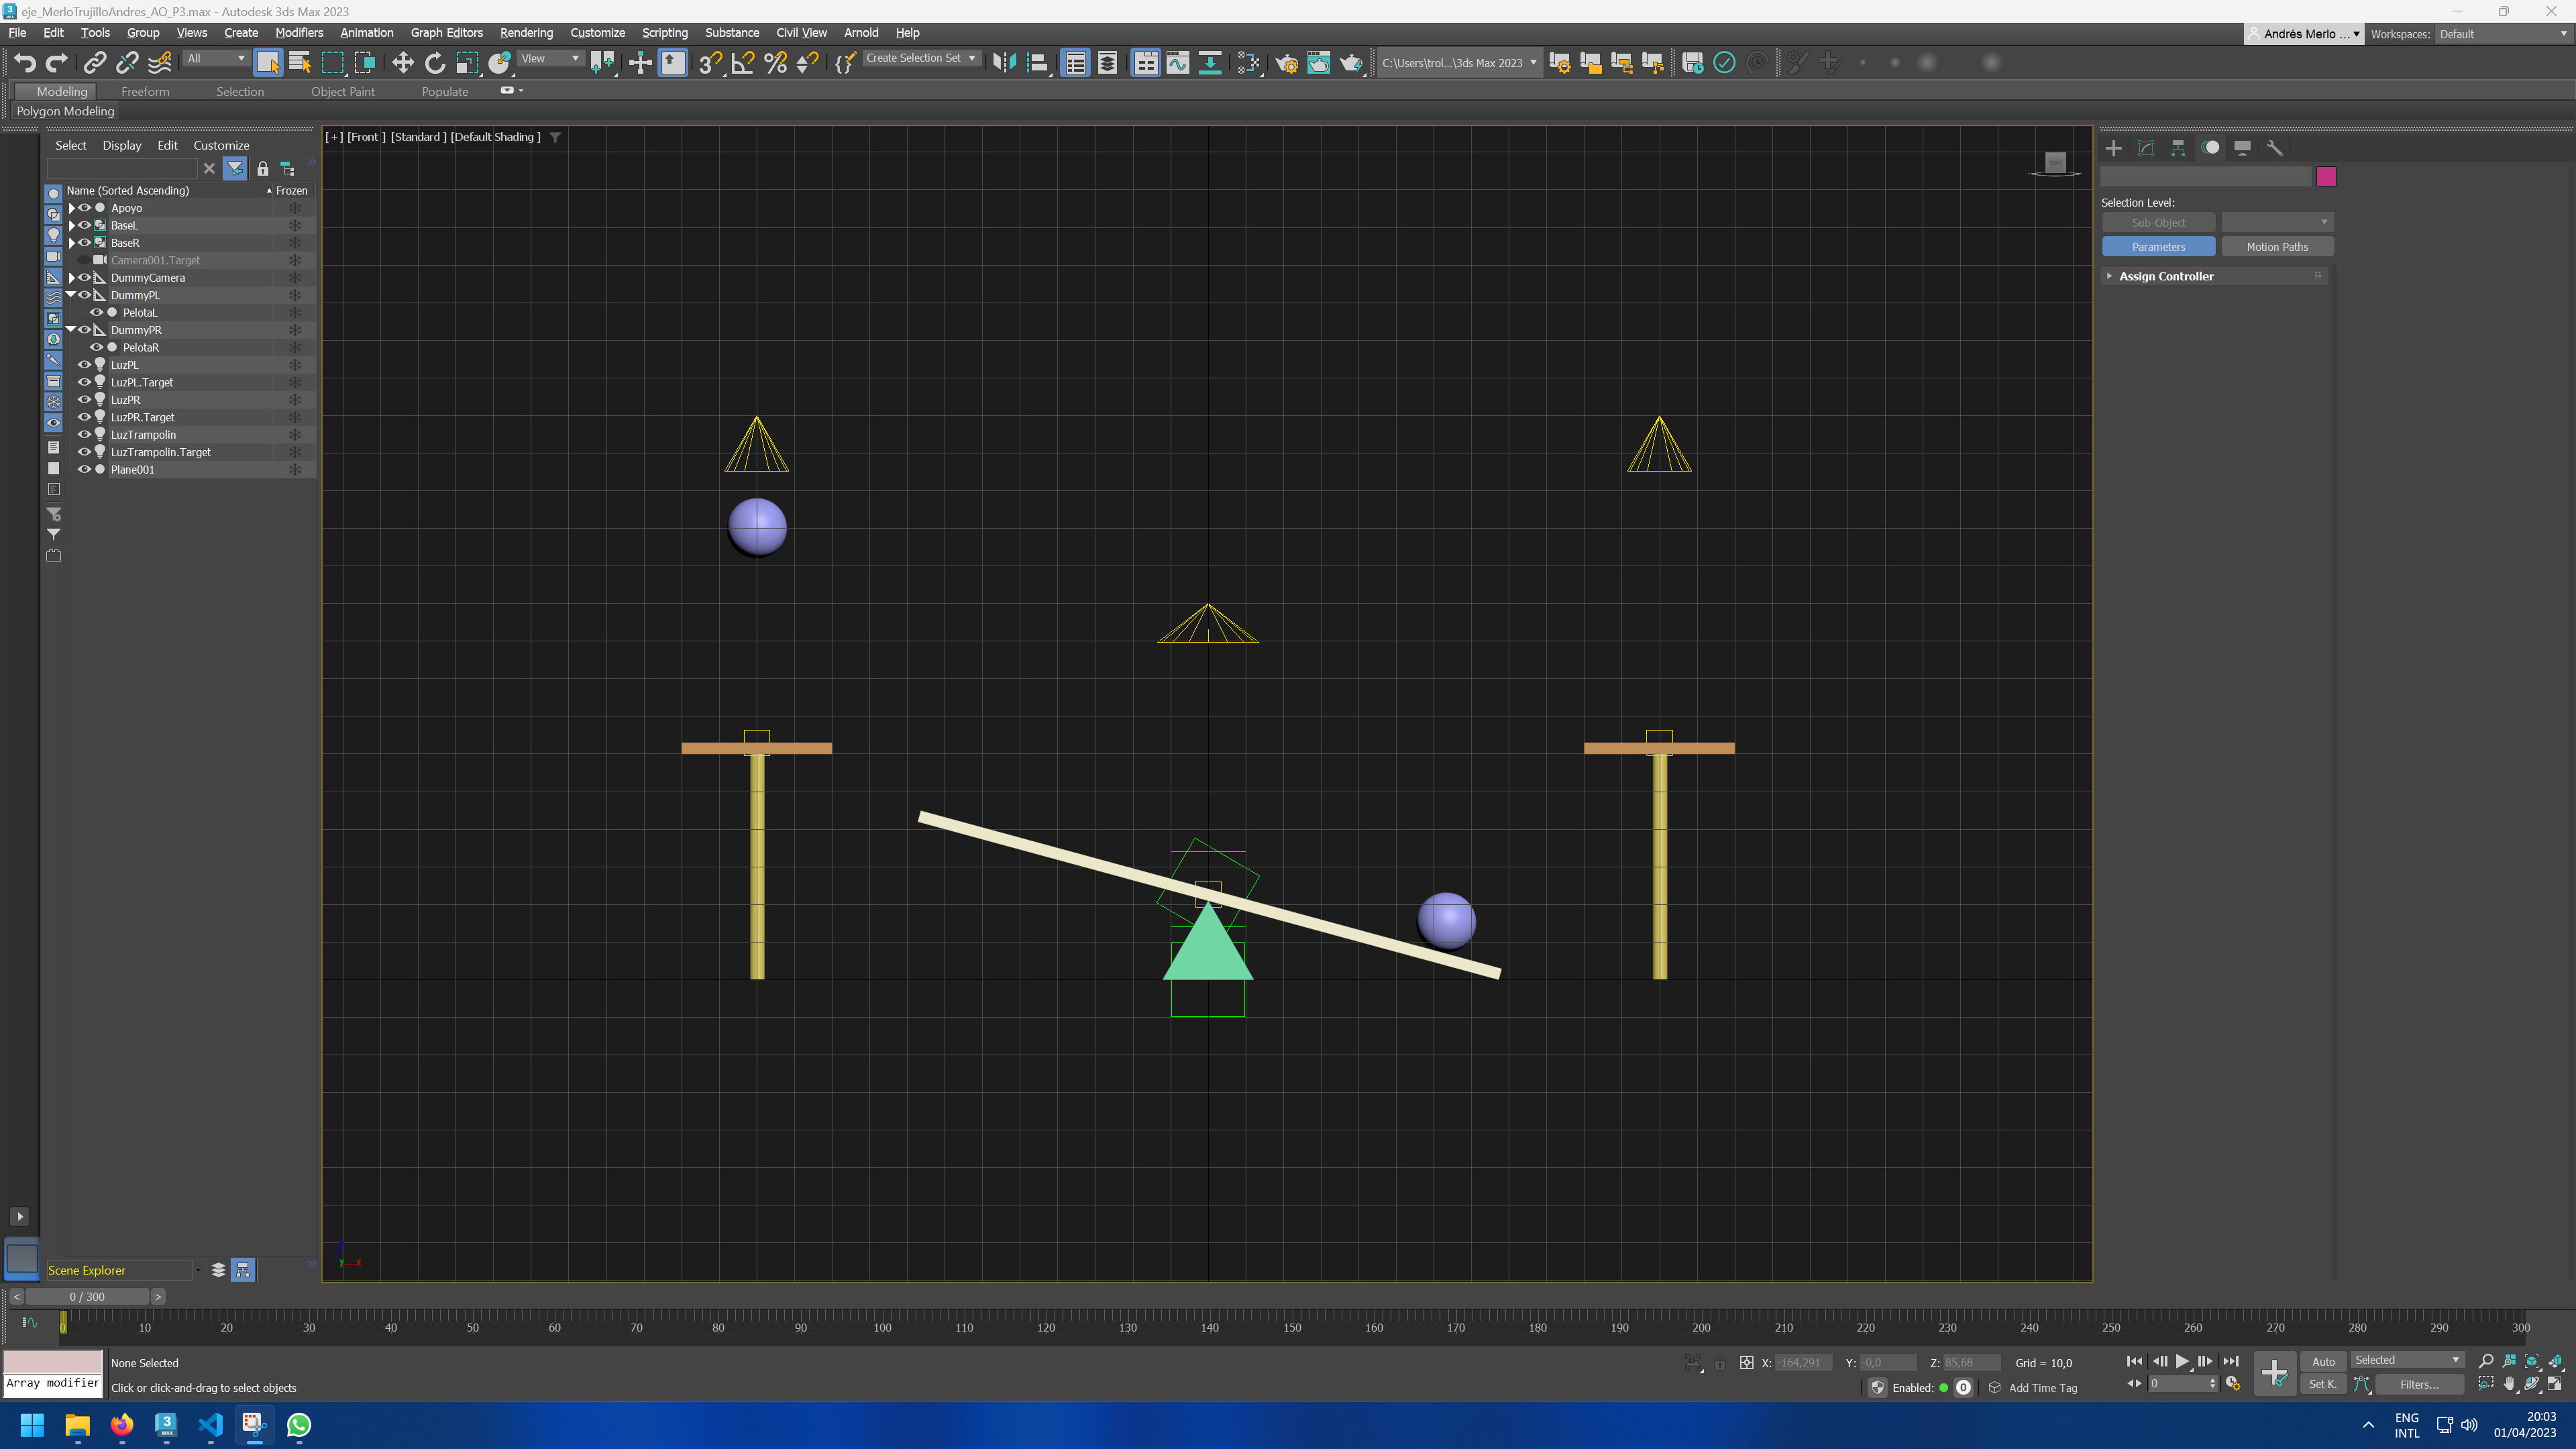
\includegraphics[width=\textwidth]{imagenes/Ejercicio 1/keyframes/0.png}
%         \caption{Pelotas en el instante 0.}
%     \end{subfigure}
%     \hfill
%     %\par\bigskip %si se desea dejar un margen entre la imagen de arriba y de abajo
% 	\begin{subfigure}[H]{0.48\textwidth}
% 	    \centering
% 	    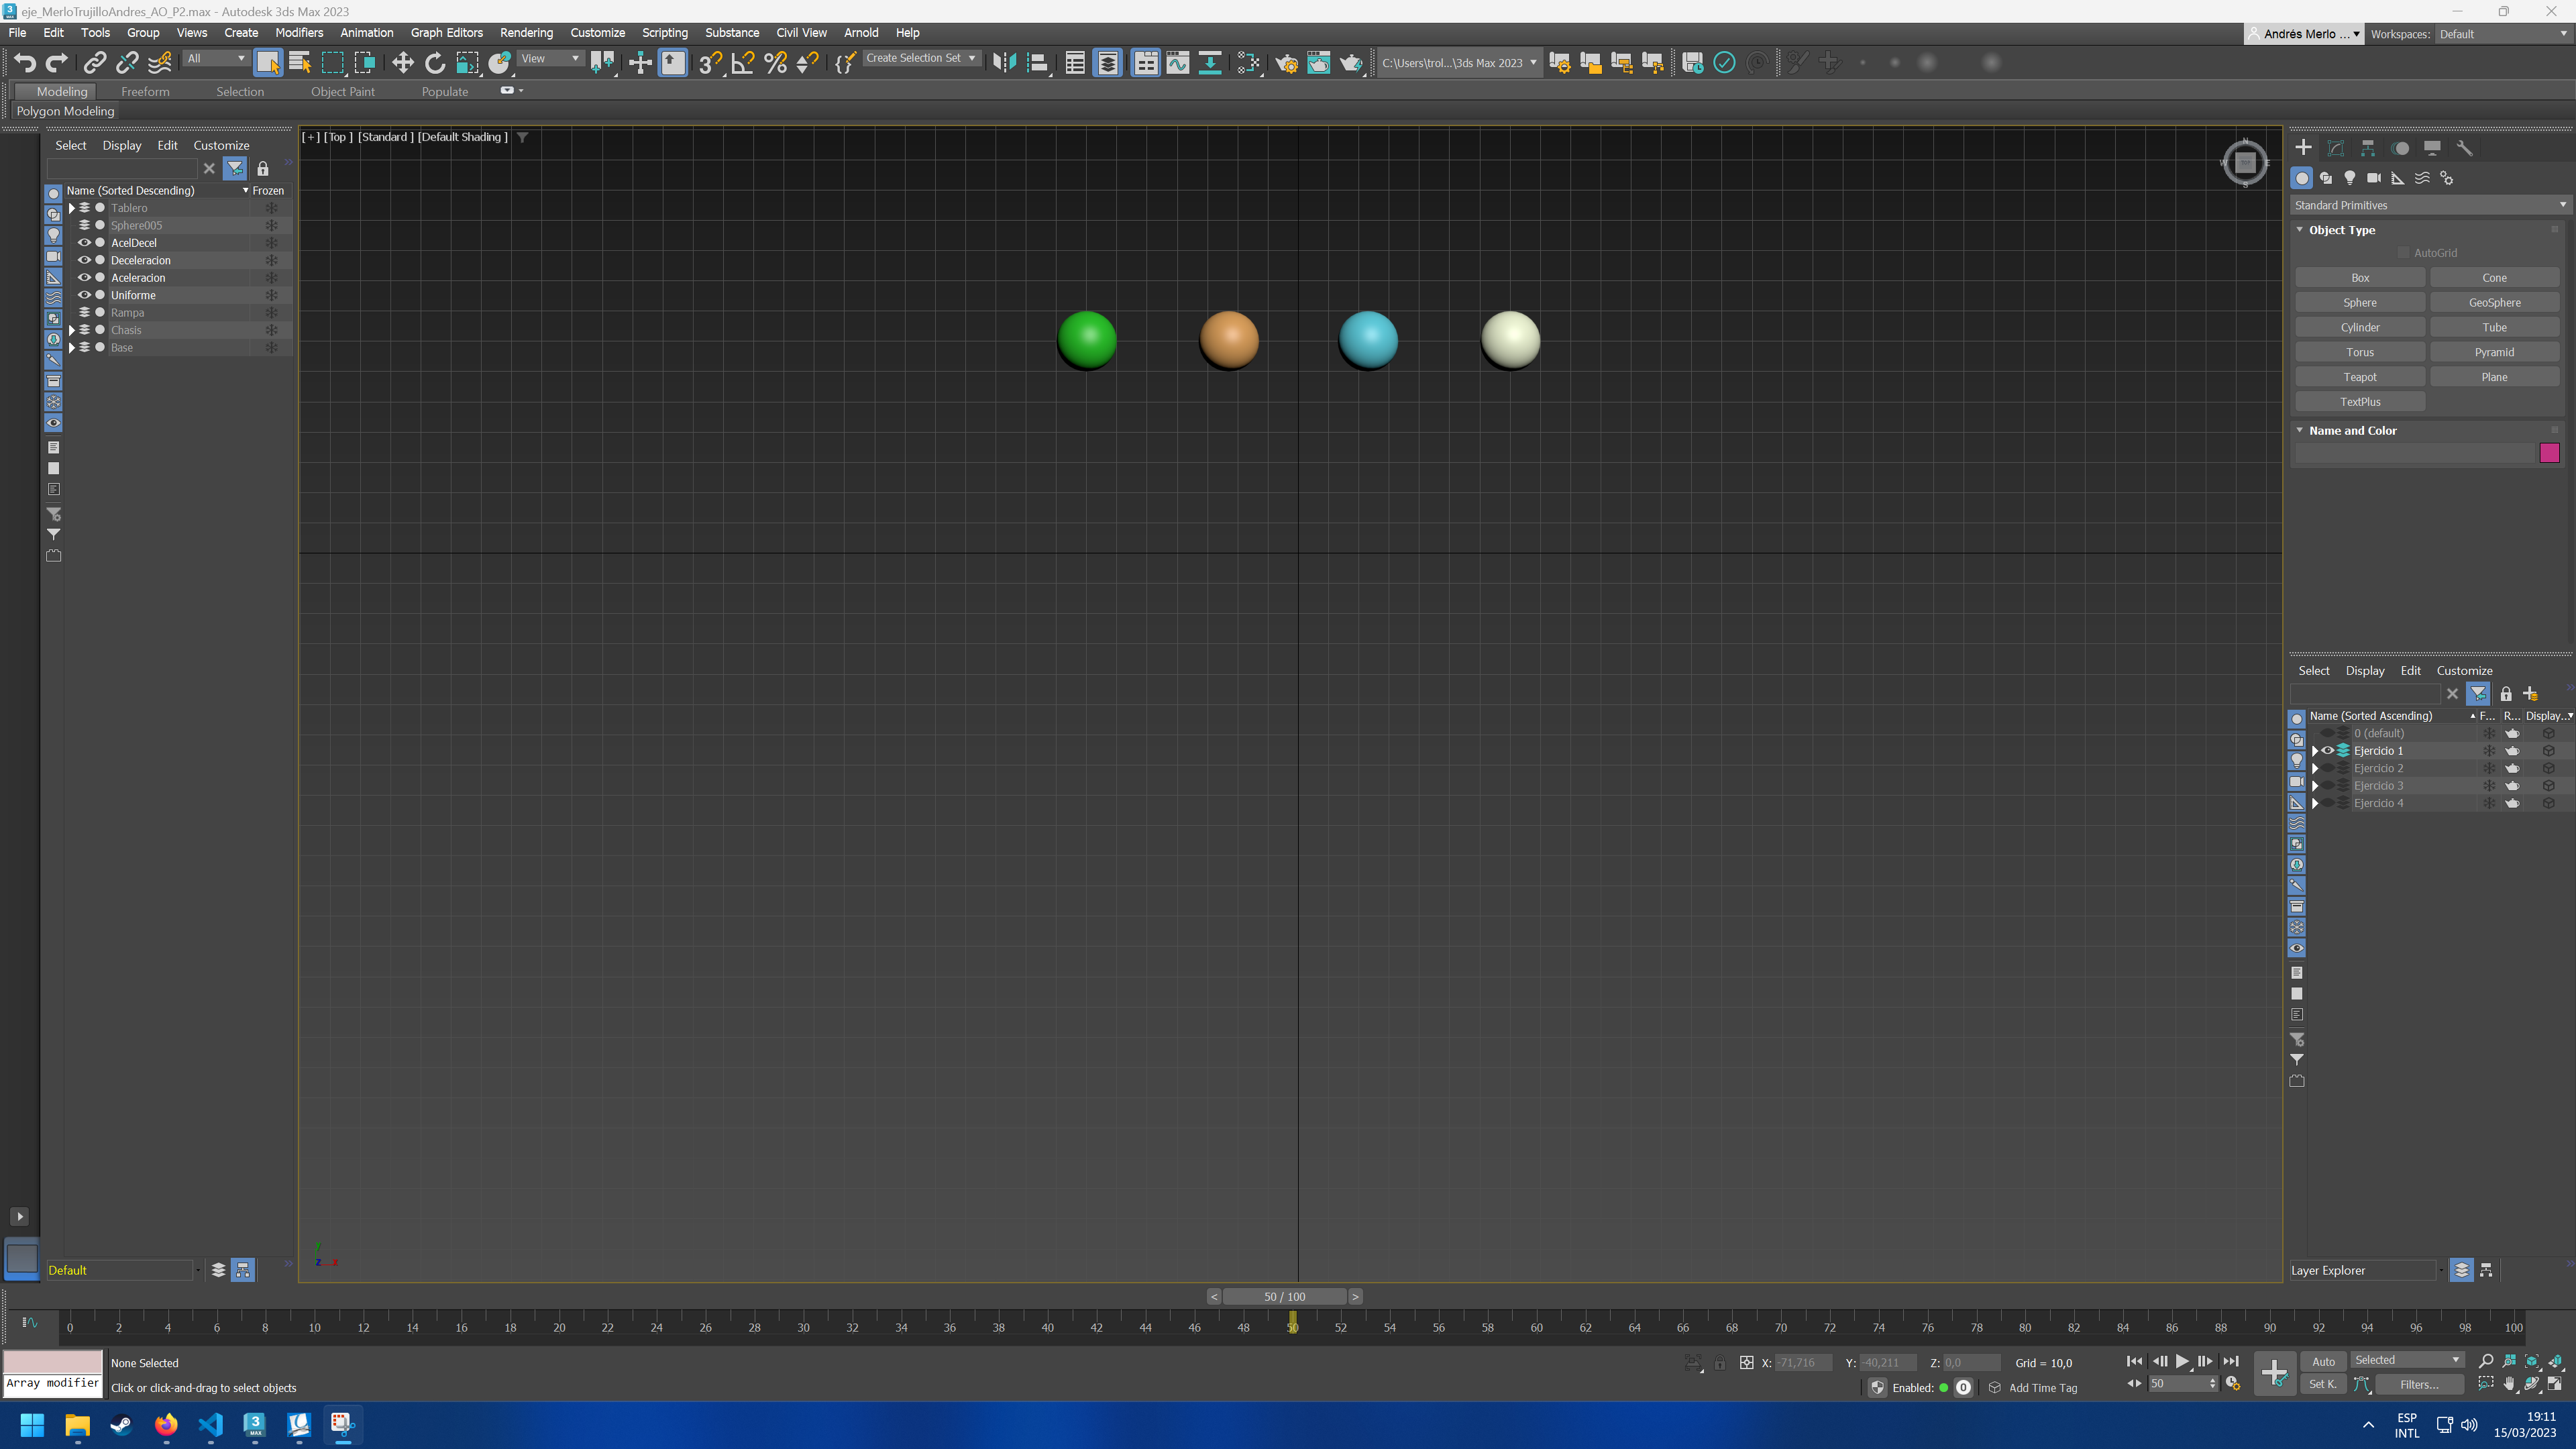
\includegraphics[width=\textwidth]{imagenes/Ejercicio 1/keyframes/50.png}
%         \caption{Pelotas en el instante 50.}
%     \end{subfigure}    
% \end{figure}

\section{Buscad un esquema general del proceso de producción 3D.}

Un ejemplo del proceso de producción es el siguiente:

\begin{figure}[H]
   \centering
   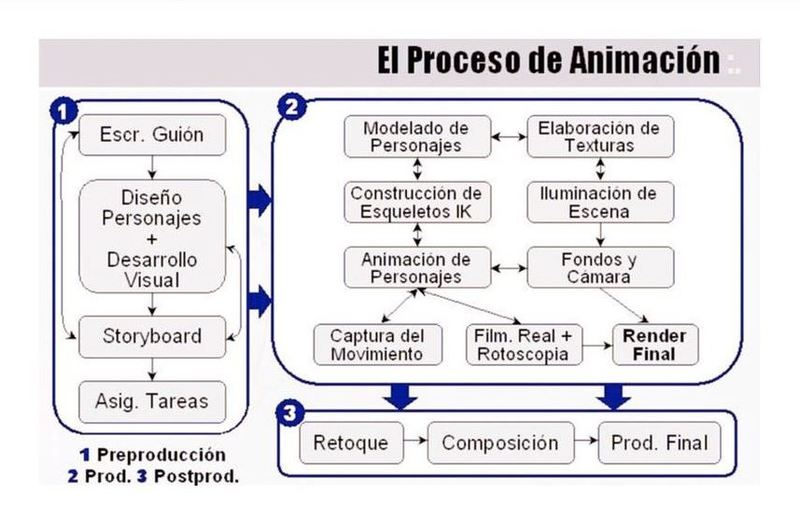
\includegraphics[width=\textwidth]{imagenes/prod.png}
   \caption{Etapas del proceso de producción 3D.}
   \vspace{10pt}
   \footnotesize{Fuente: \url{https://www.renderforest.com/es/blog/3d-animation}}
\end{figure}


Voy a dividir cada pregunta en subsecciones:

\subsection{Describid las etapas brevemente.}
Las etapas se dividen en: preproducción, producción y postproducción.

El proceso de preproducción consiste en escribir el guion y realizar \textit{storyboards}, que son bocetos que permiten plasmar la idea del guion y sus distintas escenas, junto a la apariencia de los personajes \cite{diapos}.

Las etapas de la producción 3D son:

\begin{itemize}
    \item \textbf{Modelado: }Se generan la geometría de los objetos que van a intervenir en la escena, desde los personajes hasta la vegetación de alrededor \cite{uclm}.
    \item \textbf{Rigging: }Se construye un esqueleto al personaje para que pueda moverse y cambiar de expresión \cite{animum}.
    \item \textbf{Materiales y Texturas: }Se le aplica a los objetos las propiedades de luz, color, transparencia, rugosidad, etc. Esto hace que el modelo sea más realista \cite{animum}.
    \item \textbf{Iluminación: }En esta fase se ilumina la escena mediante distintos puntos de luz, controlando parámetros como: posición de la luz, temperatura de color, \dots \cite{animum}
    \item \textbf{Animación: }Consiste en dar movimiento (``dar vida'') a los modelos de la escena, creando la ilusión de movimiento y de que los personajes sienten \cite{animum}.
    \item \textbf{Render: }Fase en la que se genera las imágenes finales que componen la animación mediante diversos cálculos, como el de iluminación.
\end{itemize}

Y el proceso de postproducción consiste en modificar las imágenes obtenidas de la renderización y aplicarles diversos filtros y efectos para obtener la imagen final \cite{uclm}.

\subsection{¿Es un proceso lineal, cíclico o mixto?}
Es un proceso mixto, ya que si nos fijamos en la imagen anterior, hay etapas en preproducción y producción que siguen ciclos, haciendo alusión a que se pueden refinar dichas etapas aún más. Un ejemplo claro de esto es cuando se realiza un personaje y se desea hacer algún cambio para que sea más acorde a su personalidad.

Mientras que en postproducción son etapas lineales, ya que una vez realizada la etapa anterior se realiza la siguiente. Esto no implica que pueda ser necesario volver a una etapa anterior para corregir o mejorar algún defecto.

En conclusión, el proceso de producción sigue un modelo mixto, al ser principalmente lineal, pero con matices cíclicos también.

\section{Indica en 3DS Max cómo se realizan cada una de las transformaciones anteriores (traslación, escalado, rotación). Haz una captura para cada caso.}

\begin{itemize}
    \item \textbf{Traslación: }Se realiza mediante la opción \textit{Select and Move}. Aparecerá en el objeto seleccionado unas flechas para mover dicho objeto.
    
    %FOTO DE LA OPCION Y OTRA DEL OBJETO
    
    \item \textbf{Escalado: }Las opciones \textit{Select and Uniform Scale} y \textit{Select and Non-Uniform Scale} permite escalar el objeto de manera uniforme y no uniforme. Aparecerán los ejes del pivote de la figura de manera distinta, permitiendo escalarlo.
    
    %FOTACA DE ESO

    \item \textbf{Rotación: }Se realiza mediante la opción \textit{Select and Rotate}. Aparecerá una esfera con circunferencias en los tres ejes sobre el pivote de la figura.
    
    %FOTO DE LA OPCION Y OTRA DEL OBJETO
\end{itemize}

\subsection{¿Conoces alguna otra transformación que ofrezca 3DS Max y que hayamos visto en clase? Indica su nombre y haz una captura.}

Existe la opción \textit{Select and Squash}, que se encuentra en la opción de escalado, manteniendo pulsado sobre el icono, la opción de más abajo.

%foto de la opcion

Esta opción permite escalar un objeto de una manera peculiar, ya que cuando se achata por un eje, el perpendicular se agranda. Esta opción es muy útil para aplicar el principio \textit{Squash and Stretch}, visto en el tema anterior de teoría y utilizado, entre otras cosas, para animar el aplastamiento de una pelota cuando toca el suelo.

%foto de la preview.

\section{¿Cómo podríamos conseguir esta transformación?}

%IMAGEN DE LA TETERA

Se puede hacer de dos formas:

\begin{itemize}
    \item La primera es moviendo el pivote de la figura mediante la opción de \textit{Affect Pivot Only}, como se hizo para el péndulo en la primera práctica.
    
    %foto de eso
    
    \item La segunda opción es creando un objeto \textit{Dummy}, cuyo pivote se va a usar para mover la otra figura. Para ello, el objeto \textit{Dummy} debe ser padre de la figura hija, para que funcionen las transformaciones.
    %foto de eso
\end{itemize}

\section{Propón un esquema jerarquizado para representar el siguiente objeto.}

%imagen de la lampara

La jerarquía utilizada en 3ds Max es la siguiente:

%foto de la jerarquia

Y la figura tiene la siguiente forma:

%foto en varias poses de la lampara

% rescribir esta frase
Cabe destacar que para que la figura sea lo más fácil de animar o mover posible, es necesario hacer que la base sea el padre, y conforme se va subiendo cada parte de la lámpara, es un hijo, siendo la cabeza donde se pone la bombilla el hijo más profundo.

\section{Basándonos en la imagen, ¿qué dos tipos de sombras debemos diferenciar durante la creación de una escena y relacionado con el aspecto del modelo?}

%imagen sombras

Las sombras propias, que son aquellas que se proyectan sobre el propio objeto y que surgen del mismo objeto \cite{sombras}. En el ejemplo de la imagen, las sombras propias son las caras más oscuras del cubo, al ser producidas por cada uno de los cubos y ser arrojados a ellos mismos.

%imagen con sombra en color rojo

El otro tipo de sombras son las sombras proyectadas, que son aquellas que produce un objeto y se proyectan sobre otro, normalmente la superficie. En la imagen de las transparencias, se puede ver este tipo de sombra proyectada en el plano, que hace de suelo.

%imagen con sombra en color rojo

\section{Busca información sobre el algoritmo de Ray Tracing. ¿Qué relación tiene que con lo visto hasta ahora? ¿Qué problema resuelve? Propón algún ejemplo visual.}

El \textit{Ray Tracing} tiene relación con lo visto hasta ahora al ser un algoritmo utilizado para generar la iluminación, sombras y reflejos, entre otras muchas propiedades, en la escena durante el renderizado.

Intentar resolver la falta de realismo en los resultados de otros algoritmos, ya que este lanza rayos desde el \textit{viewport} de la cámara a la escena, simulando los rebotes que harían los fotones y calculando el color que tendrá cada objeto en la escena. 

%rescribir quitando esto al principio
Esto permite tener efectos de iluminación muy realistas, permitiendo reflejar otros objetos de la escena en superficies reflectantes. Además, es capaz de simular efectos como: reflexión, refracción, oclusión ambiental, desenfoque de movimiento, dispersión, etc \cite{raytracing}.

%ejemplos de rt
% fortnite https://www.eurogamer.net/digitalfoundry-2022-fortnite-massive-ue5-update-tech-analysis

\subsection{¿Qué problema tiene?}

El principal problema es que es muy costoso computacionalmente, siendo una mala opción para poder ver una aproximación en el \textit{viewport} de los programas de animación. Se puede acelerar el proceso haciendo que los rayos reboten menos veces. No obstante, las tarjetas gráficas modernas tienen integradas núcleos específicos para realizar trazado de rayos, permitiendo acelerar mucho el proceso y en algunos casos poder ver los resultados en tiempo real.

% Otro problema que tiene esta tecnica es el sonido que puede llegar a generar; es decir, cuando se dan ciertas condiciones, pueden aparecer muchos puntos de colores incorrectos en la escena, empeorando mucho la calidad. Esto se podría solucionar hacienod que el algoritmo calcule más rebotes sobre el objeto, con la desbentaja de ser mucho más costoso computacionalmente.

%imagen ruido

\section{¿Se podrían detectar fallos en la animación visualizando solamente las curvas?}

Sí se podría. Un ejemplo claro es en las caídas de objetos por la gravedad, si no se ha usado una curva de aceleración, se puede ver que no va a ser del todo correcta la animación sin necesidad de ejecutarla. Otro ejemplo es para movimientos

\section{¿Las curvas nos pueden proporcionar información sobre si un objeto está en movimiento o parado?}

Sí. Uno de los ejes de las curvas, concretamente el eje Y, representa la posición del objeto. Por tanto, esta curva representa la posición con respecto al tiempo. Entonces lo que hay que buscar en las curvas son secciones horizontales, que significan que cualquier atributo del objeto no ha variado en un tiempo.

\begin{thebibliography}{1}
    \bibitem{uclm} Modelado en proceso de producción y explicación del proceso de postproducción: \url{https://www.esi.uclm.es/www/cglez/fundamentos3D/01.02.Ciclo3D.html}
    \bibitem{animum} Explicación de las etapas en el proceso de producción: \url{https://www.animum3d.com/blog/la-produccion-3d/}
    \bibitem{sombras} Explicación de las sombras propias: \url{https://piziadas.com/2010/07/animacion-3d-luces-sombras-blogs.html}
    \bibitem{raytracing} Explicación de los distintos efectos que puede simular el \textit{Ray Tracing}: \url{https://en.wikipedia.org/wiki/Ray_tracing_(graphics)}
    \bibitem{diapos} Diapositivas Tema 3. Explicación del proceso de preproducción.
\end{thebibliography}

\end{document}
